\subsection{The CLAS12 Fast MC}

Detailed detector simulation and reconstruction of physics events at CLAS12,
based on the GEANT4, is very CPU intensive and hence time consuming due to 
the high energy and multiplicity of the Monte-Carlo events and the complexity of the detectors. 

A dynamically configurable package for fast Monte-Carlo simulation and reconstruction (FASTMC) 
has been developed for CLAS12 to allow fast studies of effects of detector resolutions 
and acceptances on various samples of Monte-Carlo events. 
Each step of the chain - simulation and track reconstruction, 
has been replaced by modules that parametrize acceptance and responses of different 
detector components.

The FASTMC package uses a configuration file provided by user, which has all relevant information,
including the resolutions and acceptances for different particles and kinematics.
The initial set of parameters was derived from calculations and are getting updated with
new simulation studies from GEANT4 CLAS12 simulation.
Sets of parameters were defined for central and forward detectors of CLAS12 and for inbending
(torus current positive, so electrons will in bend in the CLAS12 torus) and outbending conditions.
Two subroutines were called in the FASTMC package susequently to provide information
on acceptance(Accep\_Fun.F) and momentum and angular smearing of tracks (Smear\_Fun.F) in the 
CLAS12. 

\subsubsection{CLAS12 acceptance}

The parameters defining the acceptance of events are listed in the configuration 
file (confXXXX.dat):
The acceptance of $e\pi X$ events is shown on Figure \ref{fig:accept}.
\begin{figure}[htbp] %  figure placement: here, top, bottom, or page
   \centering
   \includegraphics[width=2in]{fastmc/drawcl12thetavsphi_elepim_log.eps} 
   \caption{\it Acceptances for generated DIS electrons (left) and reconstructed electrons (center)
and $\pi^+$ (right).
}
\label{fig:accept}
 \end{figure}

\subsection{CLAS12 momentum and angular smearing}

The parameters defining the smearing of particle angles and momenta 
are listed in the configuration  file (confXXXX.dat):


The resolutions are calculated using simple parameterizations obtained from GEANT4 simulation
for momentum, polar and azimuthal angles:
\begin{equation}
\sigma_p =  \frac{T_{max}}{T} \sqrt[]{(\sigma_1^p \cdot p)^2 + (\frac{\sigma_2^p}{\beta})^2}
\end{equation}

where,
$$
\sigma_{[1/2]}^p = \sigma_{[{1/2}]}^1 + \sigma_{[{1/2}]}^2 \cdot \theta + \sigma_{[{1/2}]}^3 \cdot \theta^2)
$$


$$
\sigma_\theta=\sqrt{\sigma_{1\theta}^2+(\sigma_{2\theta}/p/\beta)^2}\sin^2\theta
$$
$$
\sigma_\phi=\sqrt{\sigma_{1\phi}^2+(\sigma_{2\phi}/p/\beta)^2}
$$

The smearing due to energy loss and multiple scattering of particles in the central detector
is shown in Fig.\ref{fig:smear}.


\begin{figure}[htbp] %  figure placement: here, top, bottom, or page
   \centering
   \includegraphics[width=6in]{fastmc/drawcl12dthetavs_epi_log.eps} 
   \caption{\it Resolutions of electron polar (left) and azimuthal (cetre) angles in the forward
detector and $\pi^-$  in the central detector (right).
}
\label{fig:smear}
\end{figure}

The FASTMC allows to study effects of detector resolutions and smearing on various 
physics observables. The missing mass resolutions of $e\pi X$ is shown on
Fig.\ref{fig:epX}.



\begin{figure}[htb]
\begin{minipage}[b]{6.0cm}
 \includegraphics[width=2in]{fastmc/pipmx_forw.eps}
\end{minipage}
    \ \hspace{0mm} \hspace{0mm} \
\begin{minipage}[b]{6.0cm}
\includegraphics[width=3in]{fastmc/pipmx_cent.eps}
\end{minipage}
\caption{\it Missing mass resolutions for $e'\pi X$ sample for forward  (left) and 
large angle $\pi^+$ (right) events.
}
\label{fig:epX}
\end{figure}

The distribution of events from Lambda and Sigma decays as a function of the angle between
plains containing the $\Lambda$ and the Kaon are shown on Figure \ref{fig:KLam}.

\begin{figure}[htb]
\begin{minipage}[b]{6.0cm}
\includegraphics[width=3in]{fastmc/lambdakaonmak_lam_tmax5.eps}
\end{minipage}
    \ \hspace{0mm} \hspace{0mm} \
\begin{minipage}[b]{6.0cm}
\includegraphics[width=3in]{fastmc/lambdakaon-sepppl_lam_tmax5.eps}
\end{minipage}
\caption{\it Angle between Lambda and the Kaon for different processes, for generated (left) and reconstructed (right) distributions. The right pannel shows corresponding efficiencies  (circles)
as a function of a cut on that angle and corresponding contamination (triangles).
}
\label{fig:KLam}
\end{figure}

The Figure \ref{fig:twopi} shows the $W$ distribution calculated from the electron 
momentum (left) and using detected pions in the forward detector (center) and central
detector (right). 

\begin{figure}[htb]
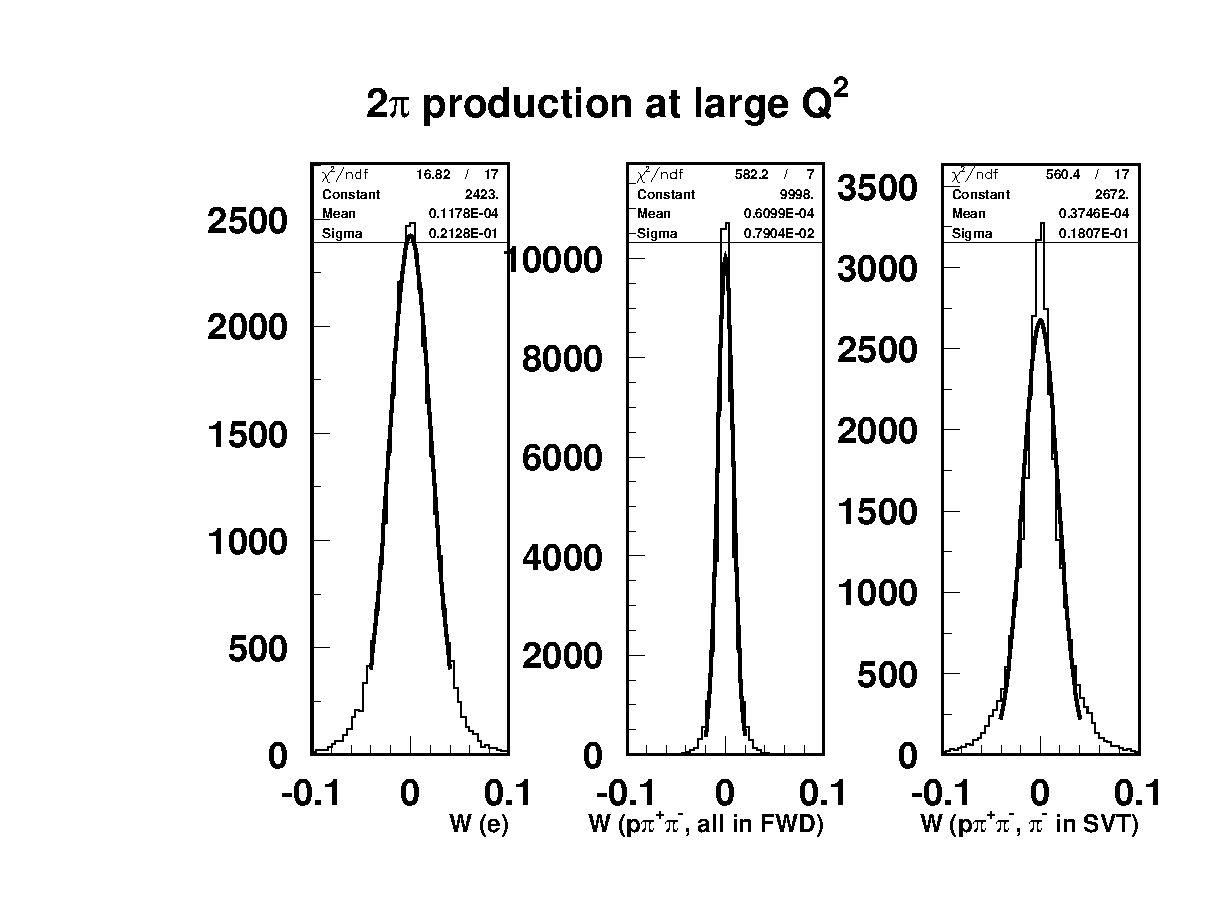
\includegraphics[width=6in]{fastmc/twopi.eps}
\caption{\it $W$-distributions for exclusive 2 pion processes in CLAS12 from FASTMC.}
\label{fig:twopi}
\end{figure}



